\documentclass[english,compress]{beamer}
\usepackage{kloeckislides}
\nonstopmode

\usepackage[normalem]{ulem}
\usepackage{pifont}
\usepackage{ifthen}

\setbeamercolor{section in head/foot}{use=structure,bg=structure.fg!25!bg}
\defbeamertemplate*{footline}{split theme}
{%
  \leavevmode%
  \begin{beamercolorbox}[wd=.5\paperwidth,ht=2.5ex,dp=1.125ex]{section in head/foot}%
    \insertsectionnavigationhorizontal{\paperwidth}{\hskip0pt plus1filll}{}%
  \end{beamercolorbox}%
  %\begin{beamercolorbox}[wd=.5\paperwidth,ht=2.5ex,dp=1.125ex]{subsection in head/foot}%
    %\insertsubsectionnavigationhorizontal{.5\paperwidth}{}{\hskip0pt plus1filll}%
  %\end{beamercolorbox}%
}


%\useoutertheme[subsection=false]{miniframes}

\setbeamertemplate{frametitle}[default][center]

\AtBeginDocument{%
  {
    \usebeamercolor{section in head/foot}
  }
  
  \pgfdeclareverticalshading{beamer@headfade}{\paperwidth}
  {%
    color(0cm)=(bg);
    color(1.25cm)=(section in head/foot.bg)%
  }

  \setbeamercolor{section in head/foot}{bg=}
}

\addtoheadtemplate{\pgfuseshading{beamer@headfade}\vskip-1.25cm}{}

\beamertemplatedotitem

\setbeamercolor{section in head/foot}{parent=palette quaternary}
\setbeamercolor{subsection in head/foot}{parent=palette primary}

\setbeamercolor{author in head/foot}{parent=section in head/foot}
\setbeamercolor{title in head/foot}{parent=subsection in head/foot}



\AtBeginSection[] {
  \begin{frame}<beamer>
  \frametitle{Outline}
  \tableofcontents[sectionstyle=show/shaded,subsectionstyle=show/show/hide]
\end{frame}
}
\AtBeginSubsection[] {
  \begin{frame}<beamer>
  \frametitle{Outline}
  \tableofcontents[sectionstyle=show/shaded,subsectionstyle=show/shaded/hide]
\end{frame}
}

\newcommand{\technicality}[2]{%
  {\strut #1\\
    \begin{beamercolorbox}[sep=1mm]{block body}
      #2
    \end{beamercolorbox}
  }%
}

\lstset{
  language=C++,
  rangebeginprefix=//\ ,
  rangeendprefix=//\ ,
}

\def\weblink#1#2{\href{#1}{\color{blue}\underline{#2}}}

\definecolor{fetch}{RGB}{227,110,35}
\definecolor{alu}{RGB}{255,188,24}
\definecolor{context}{RGB}{132,146,175}

\usepackage{keystroke}

\setbeamertemplate{navigation symbols}{}


\begin{document}
% {{{ front matter

\title{High-Performance Scientific Computing\\Lecture 1: Intro}

\date{MATH-GA 2011 / CSCI-GA 2945 $\cdot$ September 5, 2012}

\frame{\titlepage}

\begin{frame}{Today}
  \tableofcontents[hideallsubsections]
\end{frame}
% }}}
% -----------------------------------------------------------------------------
\section{About this class}
% -----------------------------------------------------------------------------
% {{{
% -----------------------------------------------------------------------------
\begin{frame}{Course Goal}

  \begin{center}
    \Large
    Slow code goes in.

    \Huge
    Speedy code goes out.
  \end{center}
\end{frame}
% -----------------------------------------------------------------------------
\begin{frame}{Define slow?}
  \begin{columns}
    \column{0.6\textwidth}
    \only<1>{
      \movie[width=\textwidth,height=0.85\textwidth,poster]{}
      {../lec1-media/ka6d-contour.webm}
    }
    \only<2->{
      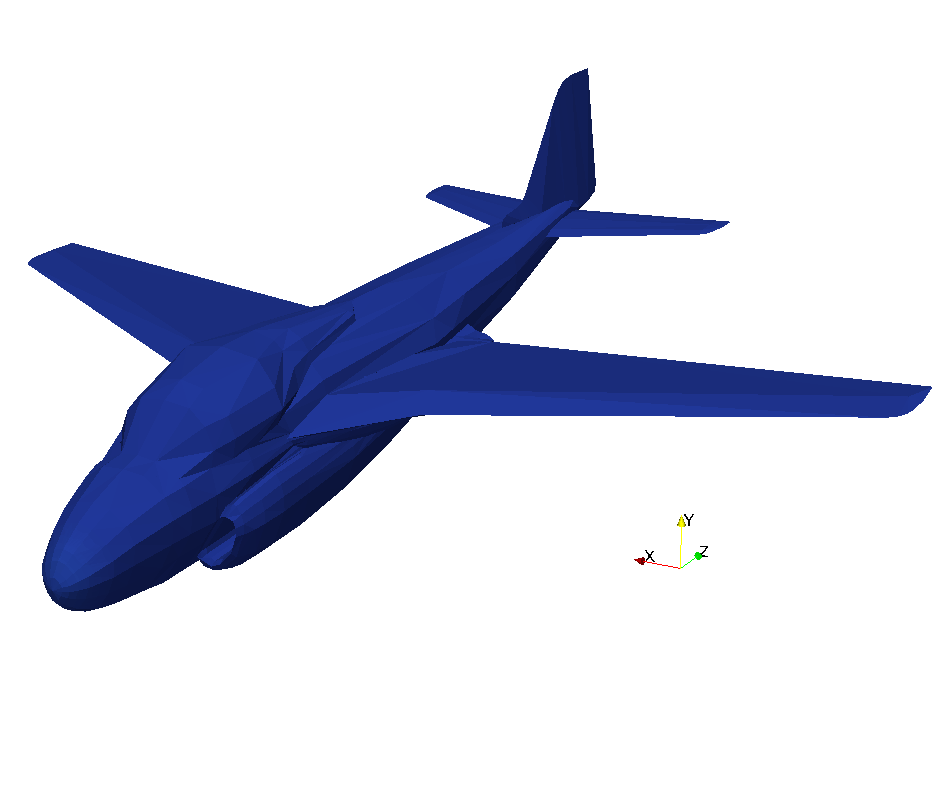
\includegraphics[width=\textwidth]{ka6d-contour.png}
    }
    \column{0.4\textwidth}
    \pause
    \begin{itemize}[<+->]
      \item Took about 30 days on a single PC.
      \item Took about a day on a GPU.
    \end{itemize}

    \uncover<+->{
      That's still pretty crude-looking.
    }

    \medskip
    \uncover<+->{
      Suppose I'd like to double the resolution. (i.e. cut the mesh
      width $h$ in half.)
    }
    \vspace{-2ex}
    \begin{itemize}[<+->]
      \item Had $K$ elements. Now?
      \item Anything else?
      \item $16\times$ the cost!
    \end{itemize}

  \end{columns}
  \uncover<+->{
    \begin{tikzpicture} [overlay]
      \node [above right=10mm of current page.south west,
        draw,drop shadow,fill=white,inner sep=5mm,thick,
        text width=6cm]
        {
          Realistic (high-fidelity) problems are big.

          \medskip
          \only<+->{
            $\rightarrow$ You'll need a bigger hammer.
          }

          \medskip
          \only<+>{%
            \textbf{%
            You'll need to know \emph{how to use} the bigger hammer.
          }
          }
        } ;
    \end{tikzpicture}
  }
\end{frame}
% -----------------------------------------------------------------------------
\begin{frame}{Course Outline}
  \begin{tikzpicture}[overlay]
    \node [above left =1cm of current page.south east,
    rotate=10,opacity=0.3,yshift=1cm] 
    { \includegraphics[width=8cm]{dictionary.jpeg} } ;
  \end{tikzpicture}
  \begin{columns}
    \column{0.5\textwidth}
    \textbf{Part 1: Do} ($\sim 4$)

    \begin{itemize}
      \item Write, run programs (C)
      \item Use tools (make, git, gdb)
      \item OpenMP, MPI, OpenCL
      \item Correctness in each
    \end{itemize}

    \medskip
    \textbf{Part 2: Understand} ($\sim$3)

    \begin{itemize}
      \item Measure and understand performance
      \item Basic machine architecture
      \item CPU machine model
      \item GPU machine model
    \end{itemize}

    \column{0.5\textwidth}
    \textbf{Part 3: Refine} ($\sim$3)

    \begin{itemize}
      \item Advanced tools \& languages
      \item Work partitioning
      \item Common patterns
      \item Load balancing
    \end{itemize}

    \medskip
    \textbf{Part 4: Apply}

    \begin{itemize}
      \item Find a project\\
        (start looking \emph{now}!)
      \item Pitch it to us (5 min)
      \item Apply what you've learned
      \item Present your work (2)
    \end{itemize}
  \end{columns}
\end{frame}
% -----------------------------------------------------------------------------
\begin{frame}{Sign-up sheet}
  \begin{center}
    \includegraphics[height=7cm]{notebook.jpeg}
  \end{center}
\end{frame}
\addimgcredit{Notebook: sxc.hu/abeall}
% -----------------------------------------------------------------------------
\begin{frame}{Survey}
  \begin{columns}
    \column{0.5\textwidth}
    \includegraphics[width=\textwidth]{question-mark.jpeg}
    \column{0.5\textwidth}
    \begin{itemize}[<+->]
      \item Home department
      \item Degree
      \item Longest program ever written?
      \item Language?
      \item Parallel?
      \item Already have a project?
    \end{itemize}
  \end{columns}
\end{frame}
\addimgcredit{Question mark: sxc.hu/svilen001}
% -----------------------------------------------------------------------------
\begin{frame}{Class web page}
  \begin{columns}
    \column{0.6\textwidth}
      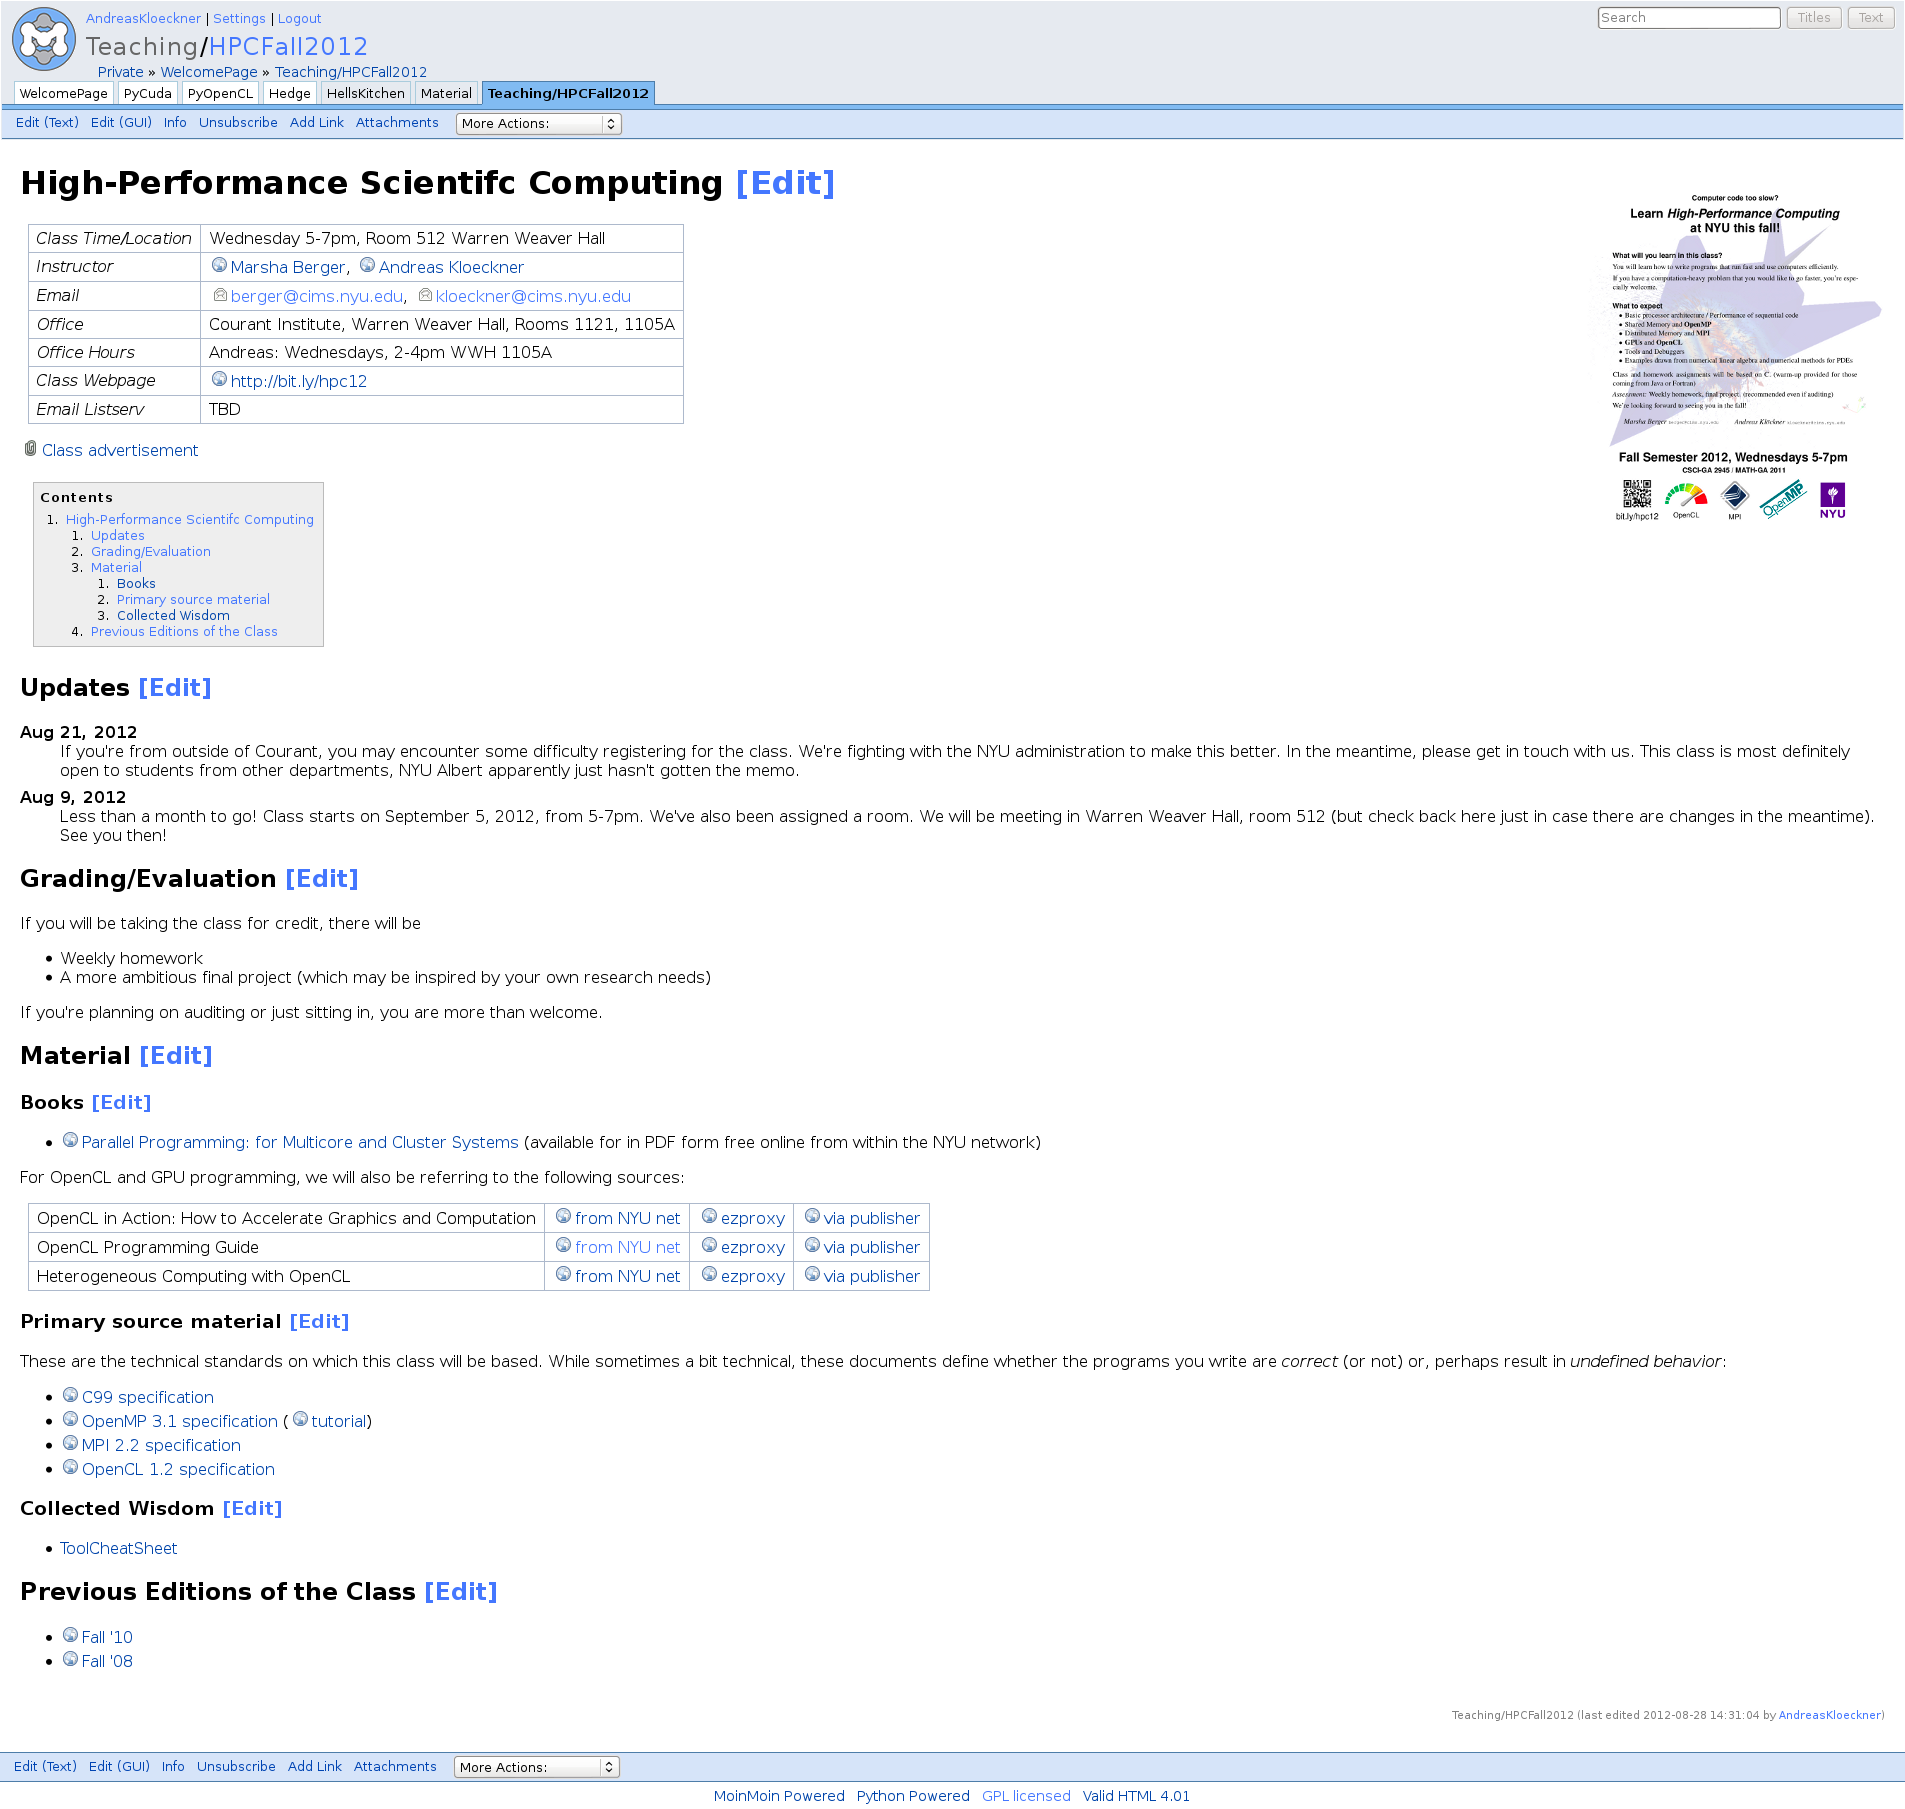
\includegraphics[width=\textwidth]{hpc-web-screenshot.png}
    \column{0.4\textwidth}
      \Huge
      \href{http://bit.ly/hpc12}{bit.ly/hpc12}
  \end{columns}
  \uncover<2>{
    \begin{tikzpicture} [overlay]
      \node [above left=10mm of current page.south east,
      draw,drop shadow,fill=white,inner sep=5mm,thick,
      text width=0.6\textwidth]
        {
          Posted: Homework set 1

          (C warm-up, git, mechanics)

          \emph{Due next week.}

          \bigskip
          Posted: Virtual machine image
          (instructions in HW1)
        } ;
    \end{tikzpicture}
  }
\end{frame}
% -----------------------------------------------------------------------------
\begin{frame}{Book 1}
  \begin{center}
    
\includegraphics[height=7cm]{rauber-ruenger.jpeg}
  \end{center}
  \uncover<2>{
    \begin{tikzpicture} [overlay]
      \node [above left=10mm of current page.south east,
      draw,drop shadow,fill=white,inner sep=5mm,thick,
      text width=0.6\textwidth]
        {
          All books accessible from NYU network.

          Links on class web page.
        } ;
    \end{tikzpicture}
  }
\end{frame}
% -----------------------------------------------------------------------------
\begin{frame}{Books 2--4}
  \begin{center}
    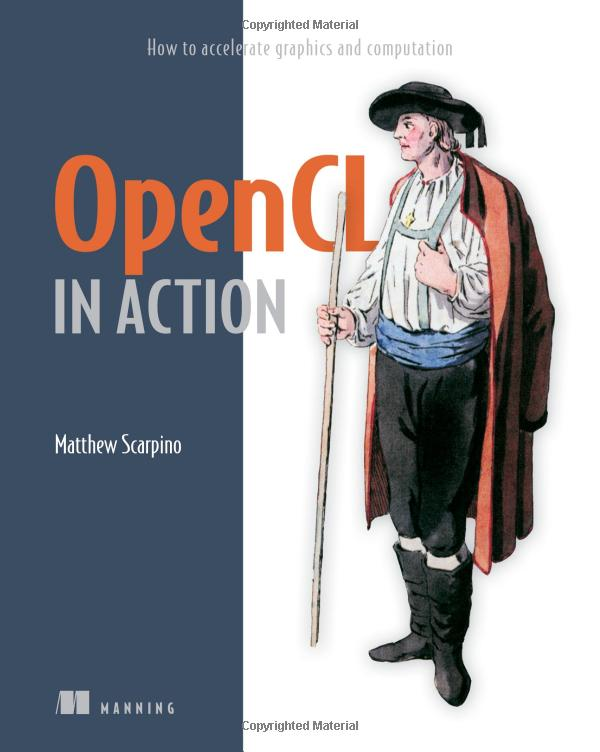
\includegraphics[height=7cm]{scarpino-opencl.jpeg}
  \end{center}
\end{frame}
% -----------------------------------------------------------------------------
\begin{frame}{Books 2--4}
  \begin{center}
    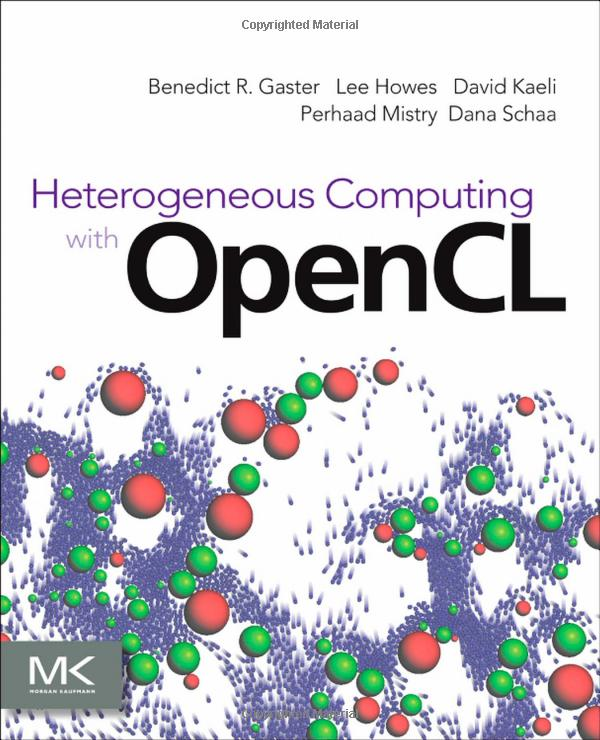
\includegraphics[height=7cm]{gaster-opencl.jpeg}
  \end{center}
\end{frame}
% -----------------------------------------------------------------------------
\begin{frame}{Books 2--4}
  \begin{center}
    
\includegraphics[height=7cm]{munshi-opencl.jpeg}
  \end{center}
\end{frame}
% -----------------------------------------------------------------------------
\begin{frame}{Grading}
  \Large
  \begin{itemize}
    \item 60\% Weekly homework
    \item 40\% Final project
  \end{itemize}
\end{frame}
% -----------------------------------------------------------------------------
\begin{frame}{Listserv}
  \begin{center}
    \Huge
    \href{mailto:hpc12@tiker.net}{hpc12@tiker.net}
  \end{center}
\end{frame}
% -----------------------------------------------------------------------------
\begin{frame}{Smile! You're on camera}
  \begin{center}
    \includegraphics[height=5cm]{camera.jpeg}

    Lecture video will be posted soon after each class.
  \end{center}
\end{frame}
\addimgcredit{Camera: sxc.hu/Kolobsek}
% }}}
% -----------------------------------------------------------------------------
\section{HPC: A look around}
% -----------------------------------------------------------------------------
% {{{
\begin{frame}{Key Realization}
  \begin{center}
    \Huge
    My program is taking too long.
  \end{center}
  \uncover<2>{
    \begin{tikzpicture} [overlay]
      \node [above left=10mm of current page.south east,
      draw,drop shadow,fill=white,inner sep=5mm,thick]
        {
          Maybe it'll get faster if I wait long enough?
        } ;
    \end{tikzpicture}
  }
\end{frame}
% -----------------------------------------------------------------------------
\begin{frame}{Moore's law}
  \begin{center}
    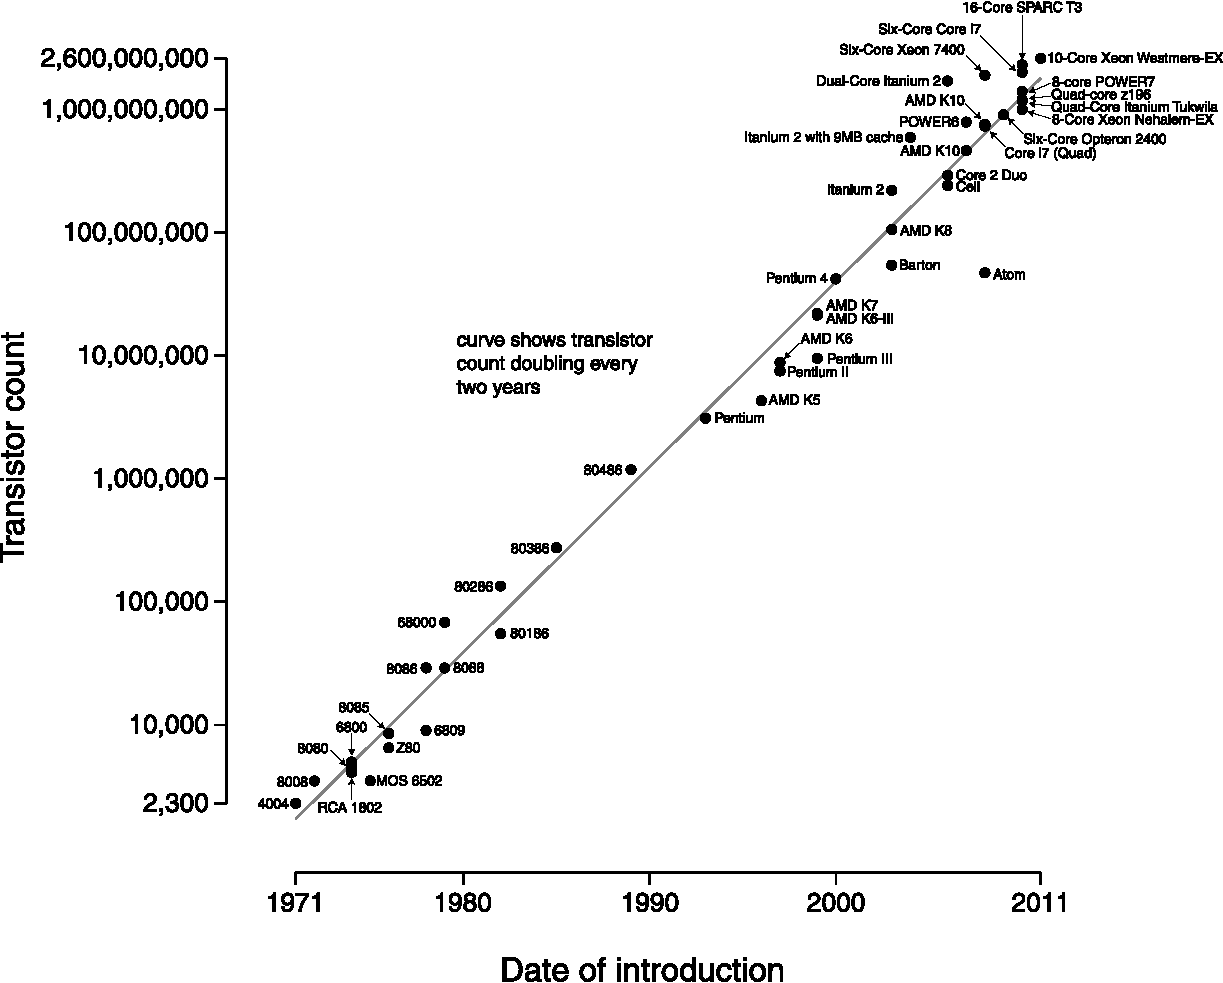
\includegraphics[height=8cm]{moores-law.pdf}
  \end{center}
  \uncover<2>{
    \begin{tikzpicture} [overlay]
      \node [above left=10mm of current page.south east,
      draw,drop shadow,fill=white,inner sep=5mm,thick]
        {
          \textbf{Issue:} More transistors = faster?
        } ;
    \end{tikzpicture}
  }
  \creditto{Wikipedia}
\end{frame}
% -----------------------------------------------------------------------------
\begin{frame}{So what does it mean?}
  \pause
  \begin{center}
    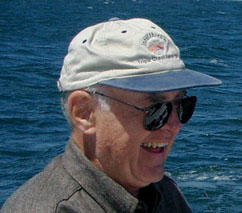
\includegraphics[height=5cm]{Gordon_Moore.jpg}
  \end{center}
\end{frame}
\addimgcredit{Gordon Moore: Wikipedia}
% -----------------------------------------------------------------------------
\begin{frame}{So what \emph{does} it mean?}
  \[
    \frac{\text{Work}}s\; = \;\text{\textbf<2>{\color<2>{red}Clock Frequency}} \; \times \; \text{Work/Clock}
  \]
\end{frame}
% -----------------------------------------------------------------------------
\begin{frame}{Dennard scaling}
  \begin{center}
    \begin{tabular}{l|c}
      \textbf{Parameter} & \textbf{Factor} \\
      \hline
      Dimension & $1/\kappa$ \\
      Voltage & $1/\kappa$ \\
      Current & $1/\kappa$ \\
      Capacitance & $1/\kappa$ \\
      Delay Time & $1/\kappa$ \\
      Power dissipation/circuit & $1/\kappa^2$ \\
      Power density & $1$
    \end{tabular}

    \bigskip
    [Dennard et al. `74, via Bohr `07]
  \end{center}

  \uncover<2->{
    \begin{tikzpicture} [overlay]
      \node [above right=7mm of current page.south west,
      draw,drop shadow,fill=white,inner sep=5mm,thick]
        {
          Frequency = Delay time${}^{-1}$
        } ;
    \end{tikzpicture}
  }
  \uncover<3>{
    \begin{tikzpicture} [overlay]
      \node [above left=10mm of current page.south east,
      draw,drop shadow,fill=white,inner sep=5mm,thick,
    text width=0.5\textwidth]
        {
          `New' problem at small scale:

          Sub-threshold leakage
          (due to low voltage, small structure)
        } ;
    \end{tikzpicture}
  }
\end{frame}
% -----------------------------------------------------------------------------
\begin{frame}{MOSFETs}
  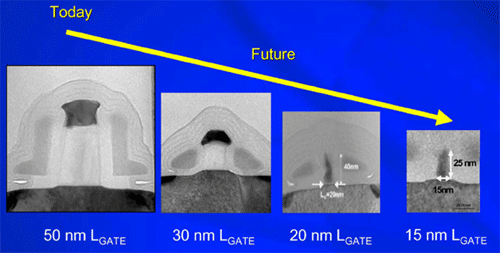
\includegraphics[width=\textwidth]{mosfet-scaling.png}
  \creditto{Intel Corporation}
  \uncover<2>{
    \begin{tikzpicture} [overlay]
      \node [above left=10mm of current page.south east,
      draw,drop shadow,fill=white,inner sep=5mm,thick,
      text width=0.5\textwidth]
        {
          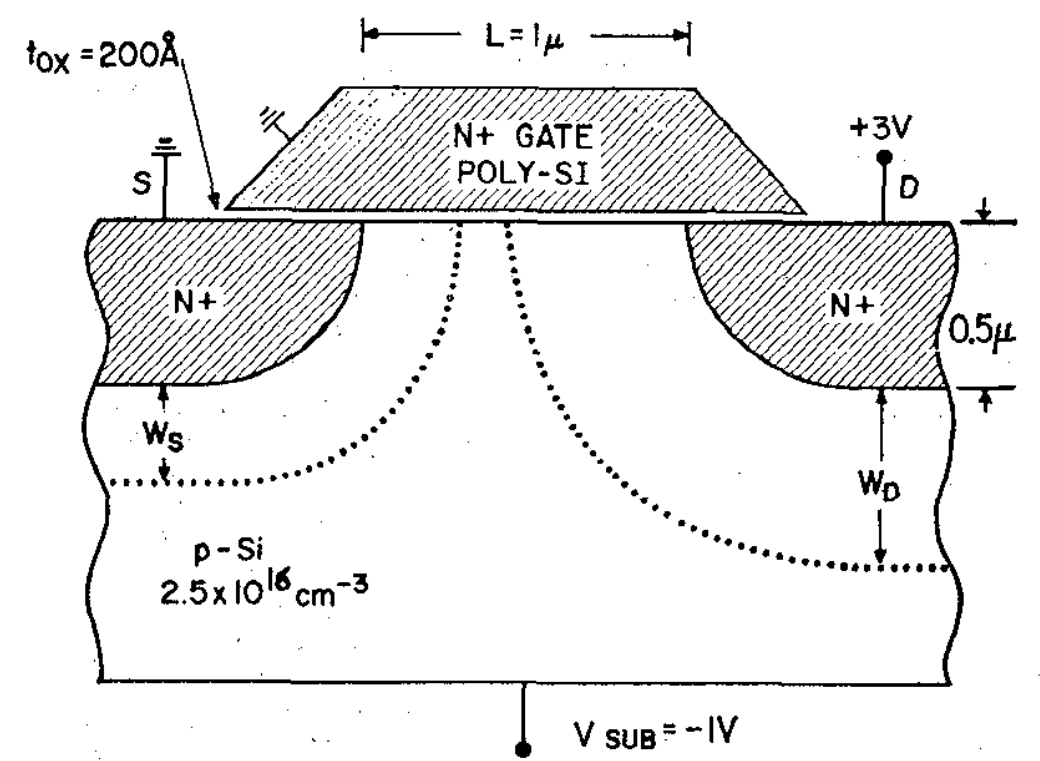
\includegraphics[width=\textwidth]{dennard-mosfet.png}

          [Dennard et al. `74]
        } ;
    \end{tikzpicture}
  }
\end{frame}
% -----------------------------------------------------------------------------
\begin{frame}{Robert Dennard}
  \begin{center}
    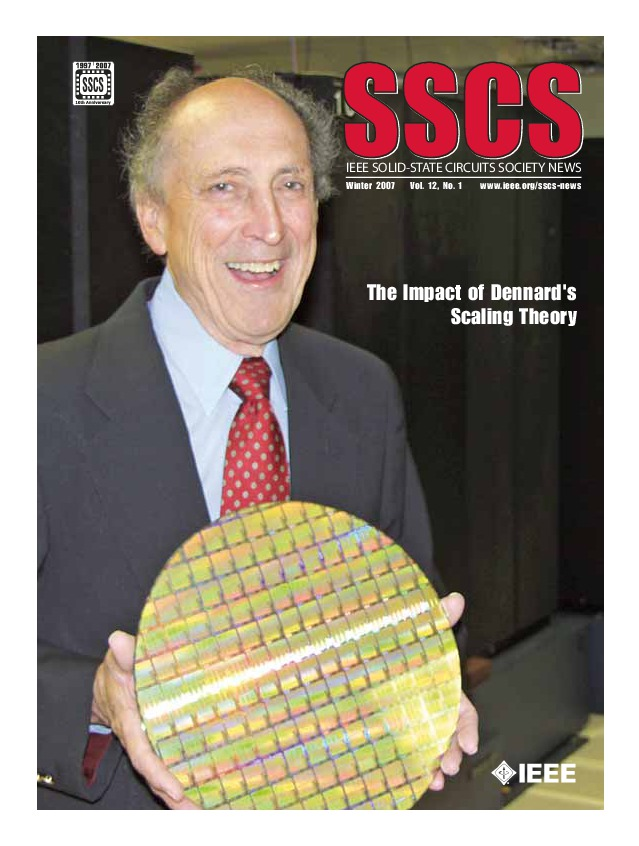
\includegraphics[height=7cm]{dennard.jpeg}
  \end{center}
\end{frame}
% -----------------------------------------------------------------------------
\begin{frame}{So what \emph{does} it mean?}
  \[
    \frac{\text{Work}}s\; = \;\tikz [baseline=(clock.base)] \node (clock) {Clock Frequency} ; \; \times \; \text{\textbf<3>{\color<3>{red}Work/Clock}}
  \]
  \uncover<2->{
    \tikz [overlay]
    \node [draw,cross out, red, very thick] at (clock) {\phantom{Clock Frequency}};
  }
\end{frame}
% -----------------------------------------------------------------------------
\begin{frame}{Instructions per clock: Intel}
  \begin{center}
    \begin{tabular}{l|l|l}
      CPU & IPC & Year\\
      \hline
      Pentium 1    &  1.1 & 1993\\
      Pentium MMX  &  1.2 & 1996 \\
      Pentium 3    &   1.9 & 1999 \\
      Pentium 4 (Willamette)&1.5 & 2003\\
      Pentium 4 (Northwood)&1.6 & 2003\\
      Pentium 4 (Prescott)&1.8 & 2003\\
      Pentium 4 (Gallatin)&1.9 & 2003\\
      Pentium D      &2 & 2005 \\
      Pentium M      &2.5 & 2003 \\
      Core 2         &3 & 2006 \\
    \end{tabular}
  \end{center}
  \creditto{Charlie Brej, \url{http://brej.org/blog/?p=15}}
\end{frame}
% -----------------------------------------------------------------------------
\begin{frame}{Instructions per clock: AMD}
  \begin{center}
    \begin{tabular}{l|l|l}
      CPU & IPC & Year\\
      \hline
      K6 II          &1.1 & 1998\\
      K6 III         &1.3 & 1999\\
      Athlon B       &1.9 & 1999 \\
      Athlon XP      &2 & 2001 \\
      Athlon 64      &2.3 & 2003\\
      Athlon 64 X2   &2.5 & 2005\\
    \end{tabular}
  \end{center}
  \creditto{Charlie Brej, \url{http://brej.org/blog/?p=15}}
  \uncover<2->{
    \begin{tikzpicture} [overlay]
      \node [above left=7mm of current page.south east,
      draw,drop shadow,fill=white,inner sep=5mm,thick]
        {
          A failure of the programming model!
        } ;
    \end{tikzpicture}
  }
\end{frame}
% -----------------------------------------------------------------------------
\begin{frame}{Processor Evolution}
  \begin{center}
    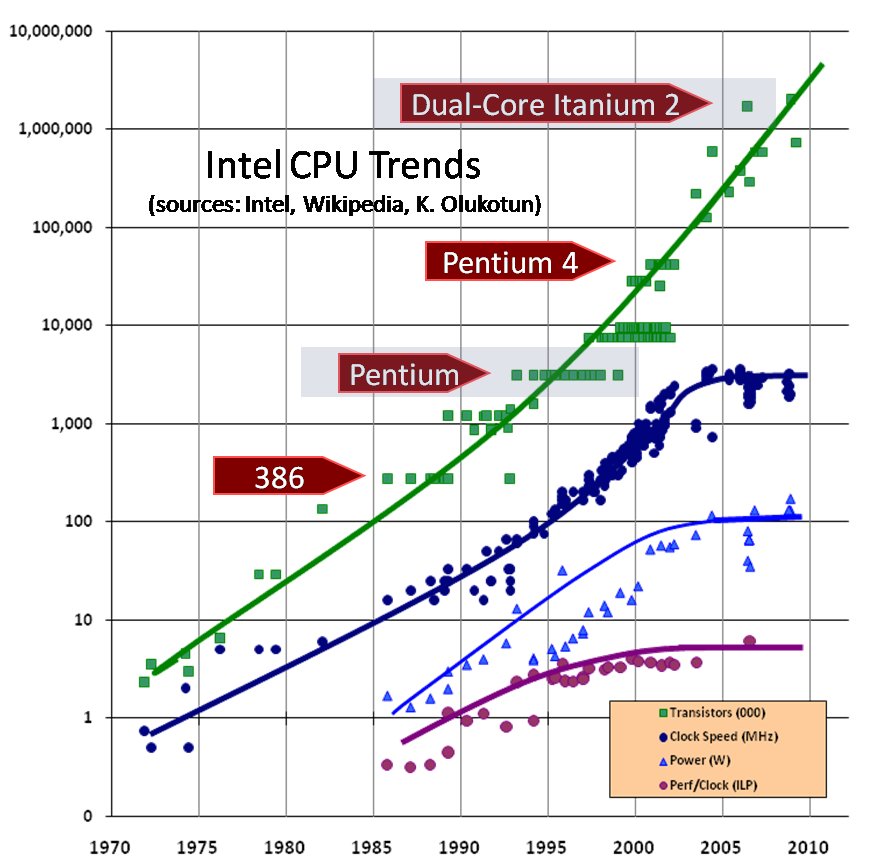
\includegraphics[height=8cm]{cpu-ilp-data.png}
  \end{center}
  \creditto{\href{http://www.gotw.ca/publications/concurrency-ddj.htm}{Herb Sutter}}
\end{frame}
% -----------------------------------------------------------------------------
\begin{frame}{Processor Evolution}
  \begin{center}
    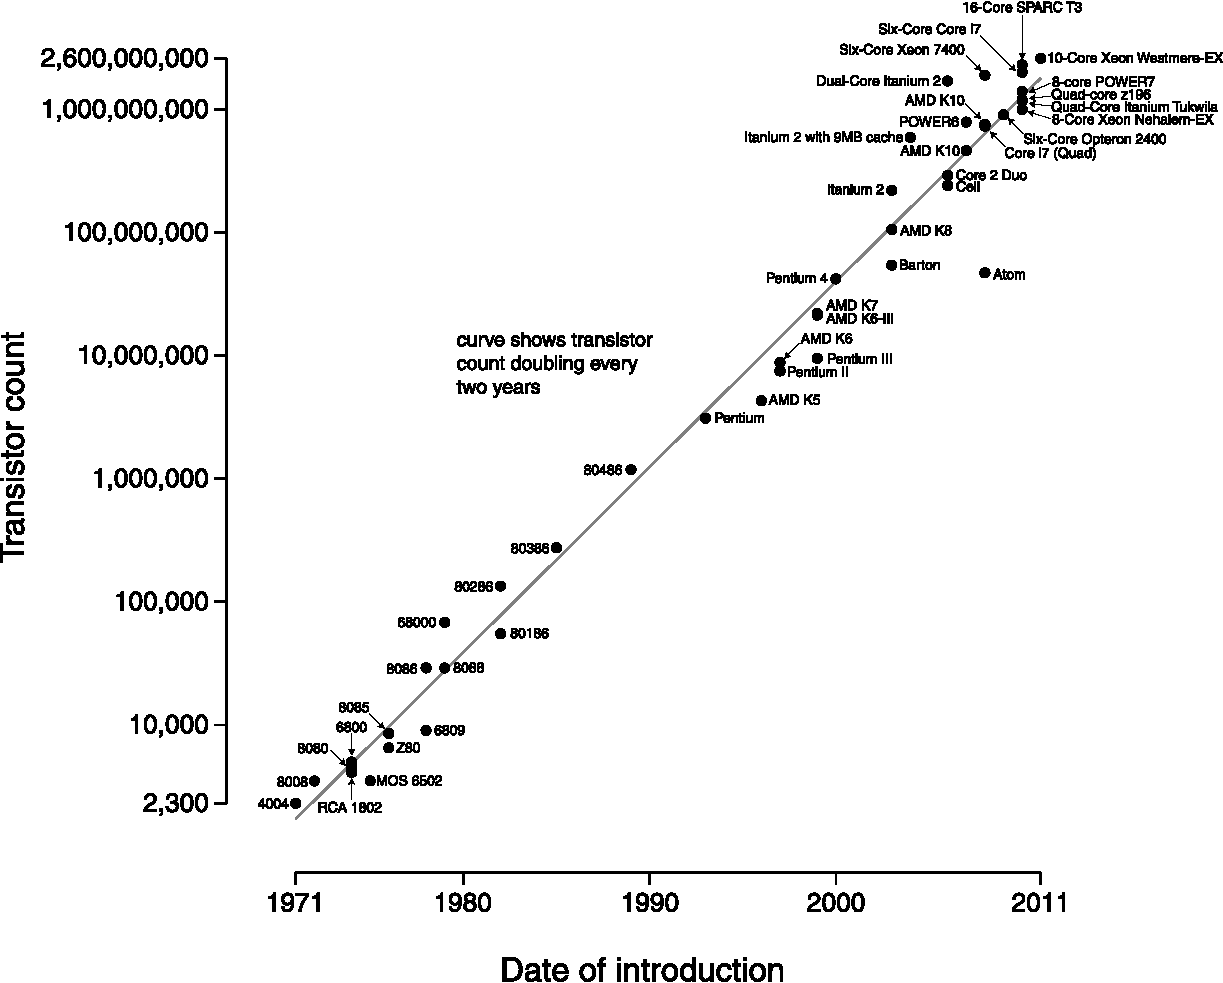
\includegraphics[height=8cm]{moores-law.pdf}
  \end{center}
\end{frame}
% -----------------------------------------------------------------------------
\begin{frame}{Parallel Programming}
  Parallel programming is \dots
  \begin{itemize}
    \item \emph{inevitable} (if you'd like maximal throughput)
    \item \emph{hard}
  \end{itemize}

  \bigskip
  \textbf{Problem:} People don't think `that way'.

  \bigskip
  ``Automatic parallelization'' has largely been a failure.

  \bigskip
  $\rightarrow$ People have to be taught to think that way.
  \hfill \uncover<2>{\textbf{:)}}
  \uncover<3>{}
  \uncover<4->{
    \begin{tikzpicture} [overlay]
      \node [above left=7mm of current page.south east,
      draw,drop shadow,fill=white,inner sep=5mm,thick,
      text width=0.5\textwidth]
        {
          \textbf{Bad news:} Parallelism might not even be
          our worst problem.

          \bigskip
          Don't just need to compute, also need to
          transmit information (to memory, say)
        } ;
    \end{tikzpicture}
  }
\end{frame}
% -----------------------------------------------------------------------------
\begin{frame}{More bad news from Dr. Dennard}
  \begin{center}
    \begin{tabular}{l|c}
      \textbf{Parameter} & \textbf{Factor} \\
      \hline
      Dimension & $1/\kappa$ \\
      Line Resistance & $\kappa$ \\
      Voltage drop & $\kappa$ \\
      Response time & $1$ \\
      Current density & $\kappa$
    \end{tabular}

    \bigskip
    [Dennard et al. `74, via Bohr `07]
  \end{center}
  \begin{itemize}
    \item The above scaling law is for on-chip interconnects.
    \item Off-chip: Similar consideration.

      Current $\sim $ Power \; \emph{vs.}\; response time
  \end{itemize}
  \uncover<2>{
    \begin{tikzpicture} [overlay]
      \node [above left=7mm of current page.south east,
      draw,drop shadow,fill=white,inner sep=5mm,thick,
      text width=0.5\textwidth]
        {
          Getting information from
          \begin{itemize}
            \item processor to memory
            \item one computer to the next
          \end{itemize}
          is
          \begin{itemize}
            \item slow (in \emph{latency})
            \item power-hungry
          \end{itemize}
        } ;
    \end{tikzpicture}
  }
\end{frame}
% -----------------------------------------------------------------------------
\begin{frame}{Summary}
  Main problems for this class:
  \begin{enumerate}
    \item Express parallelism
    \item Express communication/synchronization
    \item Analyze, understand run time

      Both theoretically and practically (by measurement)
  \end{enumerate}
  1 and 2 are \textbf{language issues!}

  \pause
  \bigskip
  A little bit of terminology:
  \begin{itemize}
    \item Speedup, Efficiency
    \item ``Amdahl's law'':

      Speed up 10\% of your program by a factor of 10?
  \end{itemize}
\end{frame}
% -----------------------------------------------------------------------------
\begin{frame}{Parallelism as a Language Question}
  \begin{center}
    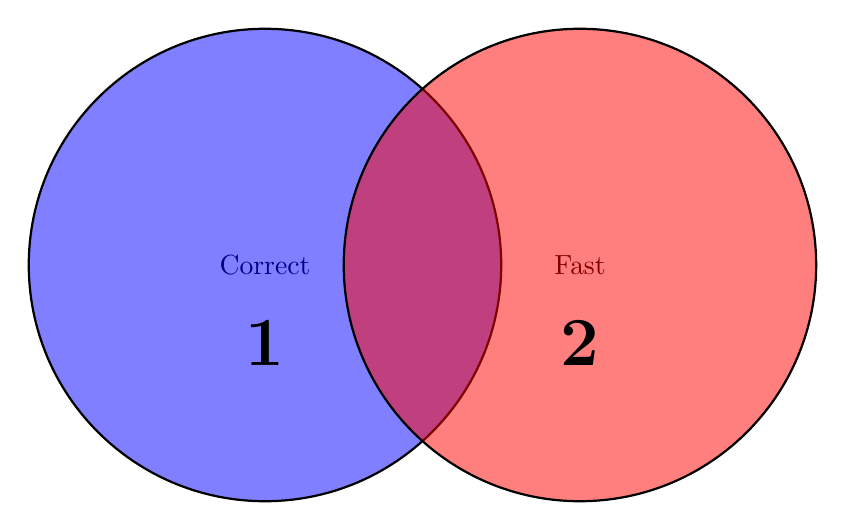
\begin{tikzpicture}
      \node at (-2,0) (correct) {Correct} ;
      \node at (2,0) (fast) {Fast} ;
      \fill [blue,opacity=0.5] (correct) circle (3cm);
      \draw [thick] (correct) circle (3cm);
      \fill [red,opacity=0.5] (fast) circle (3cm);
      \draw [thick] (fast) circle (3cm);
      \uncover<2->{ \node [yshift=-1cm] at (correct) {\Huge\bfseries 1}; }
      \uncover<3->{ \node [yshift=-1cm] at (fast) {\Huge\bfseries 2}; }
    \end{tikzpicture}
  \end{center}
  \uncover<4>{
    \begin{tikzpicture} [overlay]
      \node [above left=7mm of current page.south east,
      draw,drop shadow,fill=white,inner sep=5mm,thick]
        {
          Now let's get our hands dirty!
        } ;
    \end{tikzpicture}
  }
\end{frame}
% }}}
% -----------------------------------------------------------------------------
\section{A taste of what's to come}
% -----------------------------------------------------------------------------
% {{{
\begin{frame}
  \begin{center}
    \Huge
    Demo time!
  \end{center}
\end{frame}
% }}}
% -----------------------------------------------------------------------------
\section{Extra stuff}
% -----------------------------------------------------------------------------
\begin{frame}{HPC as a Spectator Sport}
  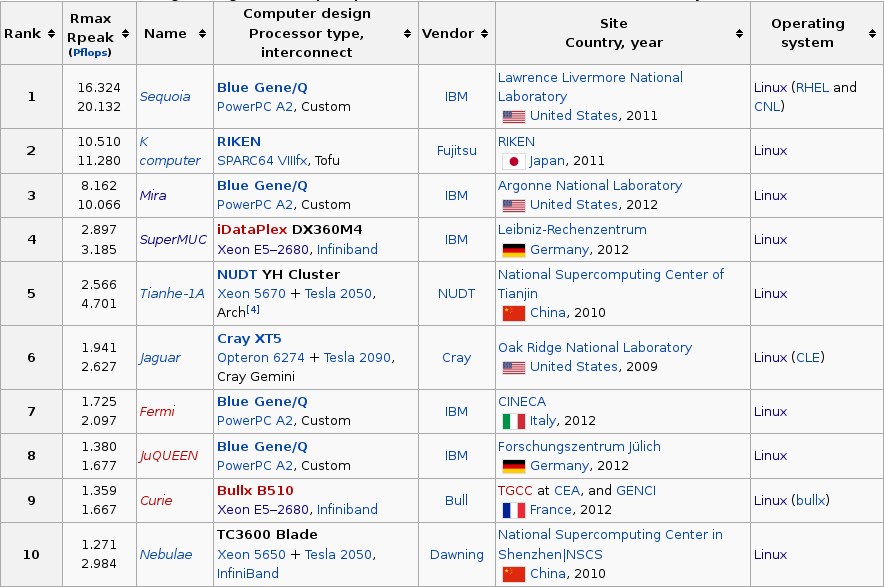
\includegraphics[width=\textwidth]{top500-list.png}
  \uncover<2>{
    \begin{tikzpicture} [overlay]
      \node [above left=7mm of current page.south east,
      draw,drop shadow,fill=white,inner sep=5mm,thick]
        {
          Know your gigas, teras, petas, and exas.
        } ;
    \end{tikzpicture}
  }
  \creditto{\url{http://top500.org}}
\end{frame}
% -----------------------------------------------------------------------------
\begin{frame}{HPC as a Spectator Sport}
  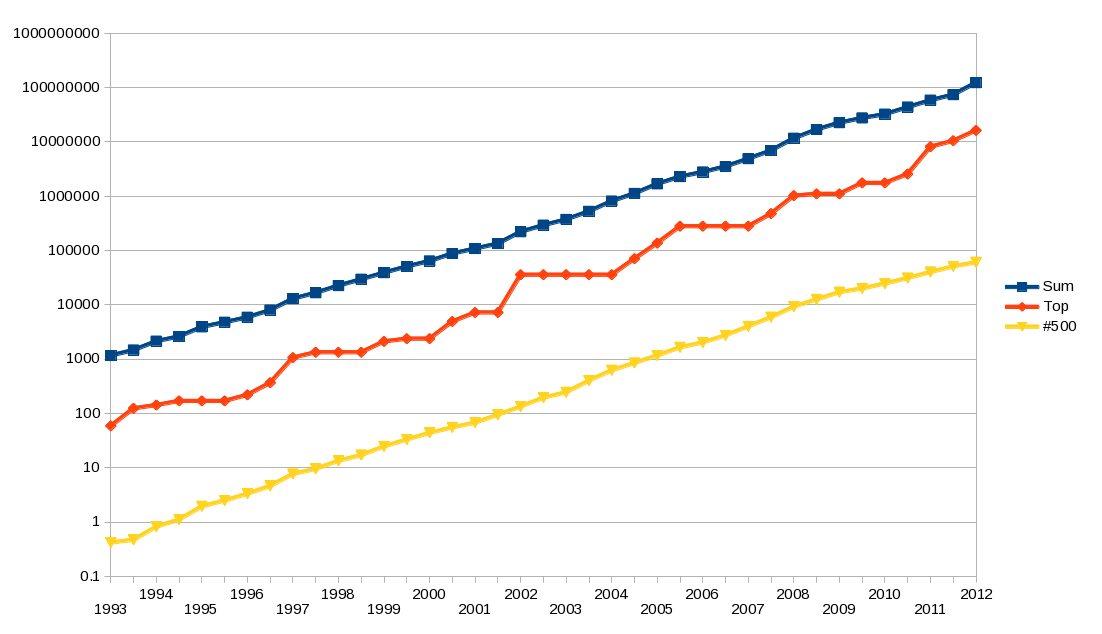
\includegraphics[width=\textwidth]{top500-performance.png}
  \creditto{\url{http://top500.org}}
\end{frame}

% Flynn: +SPMD +SIMT

\questionframe{}
\imagecreditslide

\end{document}
% vim: foldmethod=marker
